\chapter{Literature Review}
This chapter seeks to evaluate existing research in the field of rotorcraft design and obstacle avoidance strategies. To critically review some of the high level concepts in rotorcraft design, a brief evaluation is given of flight theory and how they effect design decisions for rotorcraft. After an understanding of flight theory is obtained, it is necessary to evaluate how this theory is utilised in creating rotorcraft. Armed with a better understanding of flight generation for rotorcraft, an analysis of traditional rotorcraft configurations is completed. Due to the hazardous nature of the mission environments, existing collision protection techniques are then discussed. At this point, the reader should feel confidence that the platform design is grounded with a solid understanding of existing techniques and requirements.
Now that a platform has been developed, the next step is to review some of the methods used to control multi-rotor platforms. Once stable flight methods have been evaluated and discussed, the researcher reviewed existing methods for obstacle avoidance as well as the requirements of implementing an on-board obstacle avoidance system.

\section{Flight Theory}

Although there are many different forms of flight, each form will have a very similar force diagram as seen in Figure \ref{IM_FlightForces}. 

\begin{figure}
\centering
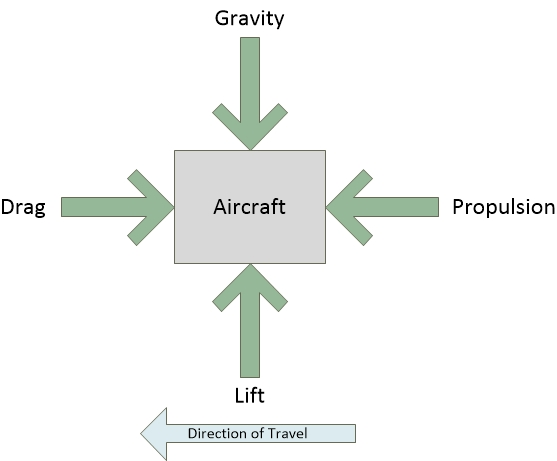
\includegraphics[height = 6cm]{Images/Literature/Flight}
\caption{Force diagram of basic components of flight}
\label{IM_FlightForces}
\end{figure}

From the force diagram it can be intuitively seen that to increase the velocity of a body in air, the lift must exceed the weight.
Weight is directly determined by the object's mass and the relevant gravity coefficient, $W = mg$. Lift counteracts this weight in an attempt to boost the body into the air. Upward acceleration is only achieved once lift exceeds weight, if they are equal the body will be in a state of hover. From the lift equation seen in \eqref{EQ_Lift} only a body with velocity can obtain lift. In a rotorcraft, the rotating blades move through the air and generate lift, thereby negating the requirement for the body to have any linear velocity. Unlike in a fixed wing aircraft if the vehicle is stationery, zero lift is generated, thus a vertical take-off is not possible. 

\begin{equation}
\label{EQ_Lift}
Lift = C_L(\frac{1}{2} \rho V^2) S
\end{equation}

To propel the body forward the propulsion must exceed the value of the drag force, which acts directly against its velocity vector. When no propulsion force is present, the craft will continue to lose speed due to drag. Similar to lift, drag varies with velocity as shown in equation (\ref{EQ_Drag}).

\begin{equation}
\label{EQ_Drag}
Drag = C_D (\frac{1}{2} \rho V^2) A
\end{equation}

The coefficient of drag ($C_D$) is determined by the objects shape and ultimately the way it interacts with the air flow. 

Figure \ref{IM_FlightForces} better describes a fixed wing aircraft, the lift and propulsion forces in a rotorcraft can be seen as the components of thrust which generate either a vertical or horizontal force. To better understand the design behind rotorcraft, the principles behind this thrust generation are discussed.

	\subsection{Fundamental Principles of Flow}
	Rotors generate thrust by pulling quiescent air through the rotor plane. The principles that best govern these flow dynamics and force generation are discussed below.
	
		\subsubsection{Continuity Equation and Bernoulli's Principle}
		Bernoulli observed that the mass flow in a closed system remains constant, as shown in \eqref{EQ_BernoulliP}. This principle states that in a closed system, the product of density ($\rho$), area (A) and velocity (v) for a flowing system will remain constant \cite{Dayle}. Based on this finding it was discovered that the mass flow of a flowing medium will follow the laws of continuity in the form of equation \eqref{EQ_Bernoulli}.
		
		\begin{equation}
		\label{EQ_BernoulliP}
		\Delta \rho Av = 0
		\end{equation} 
		
		The Bernoulli equation is a statement of the conservation of energies present in a flowing system \cite{Dayle}. Equation \ref{EQ_Bernoulli} considers a pipe with a flowing liquid and states that the energy will remain unchanged in a closed system. The sum of these energies will contain the kinetic energy of the liquid as well as the energy present through pressure. Bernoulli's equation can be rewritten in the form \eqref{EQ_Bernoulli2} to represent that any changes in pressure, can result in a change of the velocities.
		
		\begin{eqnarray}
		P_0 + \frac{1}{2} \rho v_0^2 &=& P_1 + \frac{1}{2} \rho v_i^2\label{EQ_Bernoulli}\\
		P_2 - P_1 &=& \frac{1}{2} \rho (v_\infty^2 - v_0^2)\label{EQ_Bernoulli2}
		\end{eqnarray}

		\subsubsection{Reynold's Number}
		Moving different objects in the same environment will create different results of flow, in the same breath moving the same object through different environments will also create various results of flow. Osborne Reynold attempted to mathematically determine these effects and quantify what caused a system to have turbulent flow opposed to laminar flow and vice versa. During his research he created a dimensionless constant known as the Reynold's number, as shown in equation \ref{EQ_Reynold} \cite{Reynold}. 
		
		\begin{equation}
		\label{EQ_Reynold}
		Re = \frac{\rho v L}{\mu}
		\end{equation} 
		
		In its simplest form, the Reynold's number of an object is the ratio between inertial forces ($\rho v L$) and viscous forces ($\mu$) of the gas. In a system where the viscous forces dominate ($Re ~< 10^3$), there will be laminar flow and when there are higher inertial forces ($Re >~ 10^4$) the flow will be turbulent. 
		Since turbulent flow will decrease stability and increase drag forces, Reynold's numbers have become a very important part in correctly modelling and designing aircraft \cite{Reynold}.

	\subsection{Basic Rotor Theory}
	The rotor is responsible for all the aspects of flight and generates the lift, forward propulsion and the means to control the orientation of the craft \cite{Leishman}. It is for this reason that an in depth understanding of rotor characteristics and performance was done. The original research into rotor analysis was done with helicopters, but the rotor theory basics are relevant to any rotating winged craft.
	
	Due to Newton's third law, any rotating blade will cause a a rotation in the opposite direction to that motion. This applied force will drive the vehicle to rotate around that spinning axis and creates the need for a counter torque mechanism. This is common with most rotorcraft and can be visualised in figure \ref{IM_Antitorque}, in the form of the tail rotor as seen in conventional helicopters. The quadrotor handles this by having an equal number of oppositely rotating rotors.
	
	\begin{figure}[H]
	\centering
	\includegraphics[height = 6cm]{Images/Literature/AntiTorque}
	\caption{Image Illustrating generation of Counter Torque (Taken from \cite{Heli})}
	\label{IM_Antitorque}
	\end{figure}
	
	The capability of any part of a rotor to produce lift is influenced by the local blade position and pressure at that point \cite{Leishman}.

	Angular velocity equations state that the speed of any part of the rotor varies along the length of the rotor. With the maximum velocity sitting at the rotor tip. As the rotor spins, the blade's angle of attack shifts. This angle is defined as an azimuth angle ($\psi$) and is measured relative to air flow. The azimuth angle is 0\textdegree down stream and sits at 180\textdegree when it faces directly upstream. As the rotorcraft adds a horizontal component to its hover or vertical flight, the relative speed of the individual rotor segments now adheres to equation \eqref{EQ_TipSpeed}.  As visualised in figure \ref{IM_TipSpeed}, the relative velocity at the any part of the rotor is affected by the azimuth angle of the blade ($\psi$), translational speed of the craft ($V_{\infty}$), angular speed of the rotor ($\Omega$) and the considered distance along the rotor blade (r) \cite{Leishman} \cite{RotorCraftHand}. 

	\begin{figure}[H]
		\centering
		\includegraphics[height = 6cm]{Images/Literature/TipSpeed}
		\caption{Velocity components of a rotor \cite{Leishman}}
		\label{IM_TipSpeed}
	\end{figure}
		
	\begin{equation}
	\label{EQ_TipSpeed}
	V_{r} = \Omega r + V_{\infty}\sin(\psi)
	\end{equation}
	
	What this relationship shows is that during forward flight the tip velocity, relative to the ground, changes even if the rotor rotates at a constant speed. This complicates the rotor dynamics at higher speeds and limits the top speed of the craft. On the retreating edge ($\psi = 270$\textdegree $\therefore sin(\psi) = -1$) if $\Omega r <= V_{\infty}$ the rotor would effectively be going backwards and the helicopter is at risk of stalling out, this is known as a stall condition \cite{Leishman} \cite{RotorCraftHand}, while the advancing edge is reaching its maximum speed by approaching Mach conditions and sever instability.

	\subsection{Momentum Theory and Thrust Basics}
	
	As mentioned above the rotors of a rotorcraft are responsible for generating all the forces that manoeuvre the vehicle. These forces are induced by pushing air through the rotor disk. With a fixed wing aircraft the analysis of the blades is simplified because the only air flow produced is from the translational velocity of the entire craft. Analysis of blade performance in a rotorcraft can be more challenging as the rotation of the blades must be considered along side the overall speed of the vehicle. As the craft manoeuvres in space, the air flow through the rotor has significant complexities which complicates the analysis. Since the rotorcraft is expected to perform in a variety of flight styles it is important to understand these models, and their flaws. 
	
	To simplify, initially consider a helicopter in a hovering state (Weight(W) = Thrust(T)). Figure \ref{IM_MomentumTheoryAirFlow}, taken from \cite{Leishman}, helps visualise the induced air flow by showing how the rotor smooths out the air by forcing it through the disk area. This more uniform air creates an edge known as the slipstream or wake boundary, with the surrounding air remaining dormant \cite{Leishman}. Inside the wake boundary, the average velocity of the air is tangible and effective, where outside the slipstream edge, the average air velocity is negligible and obsolete. The force required to push that mass of air through the disk space is, by Newton's third law, returned by the air unto the rotor. Thus giving the rotor blades a thrust component.
	  
	\begin{figure}[h]
	\centering
	\includegraphics[height = 8cm]{Images/Literature/MomentumTheoryAirFlow}	
	\caption{Visualisation of Induced Air Flow Through A Rotor \cite{Leishman}}
	\label{IM_MomentumTheoryAirFlow}
	\end{figure}
	
	Rankine-Froude's Momentum Theory looks at this induced velocity as well as the displacement of air through the propeller, and attempts to quantify the induced thrust. While figure \ref{IM_MomentumTheoryAirFlow} helps visualise the principle, the variable naming convention for the equations is shown in figure \ref{IM_MomentumTheoryHover} below. 
	Labels 0, 1, 2 and $\infty$ refer to the locations of quiescent flow, inflow directly before the rotor, airflow immediately after the disk and the slipstream\footnote{Generally far wake is considered as 1 full rotor diameter distance away \cite{Leishman}.} or far wake condition respectively.
	The velocities are shown as the induced velocity in and out the rotor ($v_{i}$), the far wake velocity ($v_{\infty}$) and finally $v_{0}$ represents the zone with zero flow rate. There is no velocity jump across the rotor, the energy being fed into the system by the rotor is represented by a pressure change.
	
	\begin{figure}[h]
	\centering
	\includegraphics[height = 8cm, angle=360]{Images/Literature/MomentumTheoryHover}			%Must show both air flow as well as far stream and such
	\caption{Momentum Theory in Hover (Adapted From \cite{Leishman})}
	\label{IM_MomentumTheoryHover}
	\end{figure}
	
	As described above, it is by forcing the air through the disk that lift is generated. The mass flow rate of this air can then be described by (\ref{EQ_MassFlow}), where ($\rho$) is the density of air and A is the area of one full blade rotation. The rate at which this mass of air is displaced becomes a crucial variable in rotor dynamics and is directly proportional to thrust (T). This relationship can be quantified as shown in (\ref{EQ_ThrustBasic}). Thrust can also be calculated by finding the difference in pressures over the rotor disk as in (\ref{EQ_ThrustPressure}). Since acceleration is the difference in $v_\infty$ and $v_0$, \eqref{EQ_ThrustMass} can also be obtained.
	
	\begin{eqnarray}
	\dot{m} &=& \rho A v_{i}\label{EQ_MassFlow}\\
	T &=& \dot{m}a\label{EQ_ThrustBasic}\\
	T &=& A(P_2 - P_1)\label{EQ_ThrustPressure}\\
	T &=& \rho A v_{i} (v_\infty - v_0)\label{EQ_ThrustMass}
	\end{eqnarray}
	
	Equation \eqref{EQ_ThrustMass} demonstrates the negative effect of having active ambient air. This could be caused by surrounding turbulent airflow, wind or even translational movements and will need to be considered in the controller design.

	\subsection{Disk and Power Loading}
		\subsubsection{Disk Loading}
		Disk loading (DL) is a term seen often in the world of rotorcraft, it is a simple but important ratio between thrust and the area a rotating disk makes. It is represented in \eqref{EQ_DL}. Since the pressure drop across each rotor is considered uniform, the disk loading for each rotor will equate to the pressure drop across that disk.
		 
		\begin{equation}
		\label{EQ_DL}
		DL (\frac{N}{m^{2}})= \frac{T}{A} = \frac{1}{2} \rho v_\infty^2
		\end{equation}
		
		For multi-rotor craft, the disk loading is assumed uniform across all rotors \cite{Leishman}. The overall disk loading of a single rotorcraft such as a traditional helicopter will be lower than that of a multi-rotor craft of a similar size \cite{RotorCraftHand}.  Figure \ref{IM_DL} shows some examples of disk loading values for a variety of rotor configurations, as shown disk loading is also a measure of hover efficiency.
		\todo{Edit this graph to include multirotors}
		\begin{figure}[H]
		\centering
		\includegraphics[height = 6cm]{Images/Literature/DL}     
		\caption{Image representing, various Disk Loading values for varying rotorcraft (Taken from \cite{Leishman})}
		\label{IM_DL}
		\end{figure}
		
		A higher disk loading value results in larger values for induced velocities as well as the required power to hover. This means that the larger the blades, the better the efficiency. More force will be generated by pushing large quantities of air slowly, than forcing small amounts of air through at high speeds. Of course with bigger blades, comes larger rotational inertia and geometry as well as the craft being less immune to gusts and interferences. A larger blade also creates faster tip velocities, which will limit the speed of the craft severely \cite{Leishman}.
		
		
		
		\subsubsection{Power Loading}
		Power is given by the product of both Thrust and the induced velocity at the blade. It can be written as shown in equation (\ref{EQ_Power}). What this ratio shows is that the ideal power is in cubic proportion to the induced velocity at the rotor. Therefore to reduce required power the rotor's induced velocity must be small, which can be accomplished by a significant increase in disk area \cite{Leishman}.
		
		\begin{equation}
		\label{EQ_Power}
		P = 2 \rho A v_{i}^3
		\end{equation}
		
		Another important ratio is between thrust and power, it is called power loading (PL) and is shown in equation (\ref{EQ_PL}). Power loading can be seen as a measure of craft efficiency. 
		
		\begin{equation}
		\label{EQ_PL}
		PL (\frac{N}{kW})= \frac{T}{P}
		\end{equation}
		
		From equations \eqref{EQ_DL} and \eqref{EQ_PL} it can be shown that power loading is inversely proportional to disk loading. Therefore a craft with a lower disk loading will generally be a more efficient platform.

	\subsection{Electrical Power to Thrust}
	Equation (\ref{EQ_Power}) gives a quantitative approach to solving for aerodynamic power ($P_i$). If electrical power is taken as $P_e = VI$, where V is the applied voltage and I is the sourced current, with an efficiency of $\eta$ then $P_i = \eta VI$. Noting that $P_i = T v_i$ and using equation (\ref{EQ_Power}), a relationship between thrust and $P_e$ can be formed and is represented in equation (\ref{EQ_ElectricalPowerThrust}).
	
	\begin{equation}
	\label{EQ_ElectricalPowerThrust}
	T = (2\rho A)^{\dfrac{1}{3}} (\eta P_e)^{\dfrac{2}{3}}
	\end{equation}
	
	Equation (\ref{EQ_ElectricalPowerThrust}) brings to light a very important relationship which states that thrust grows at a slower rate than the electrical input power to the system.
	
	\begin{equation*}
	T \propto P_e^{\dfrac{2}{3}}
	\end{equation*}

\section{Analysis of Conventional Rotor Wing Configurations}\label{SECT_RotorConfig}

Some of the fundamental theories described above relate to the basics behind various rotor configurations and even varying flight techniques. Each different arrangement of blades introduces certain advantages and disadvantages to the system. Not every configuration will be applicable for all operations and it is important to determine what criteria are critical for the intended application.  An analysis of varying rotor configurations is done below and follows a similar trend to that seen in \cite{RotorConfig}, \cite{Bohorquez} and \cite{NewMAV}. The main weighted criterion for the discussion were listed in no particular order as:

\begin{enumerate}
	\item Flight time and efficiency
	\item Geometry and size
	\item Drone Manoeuvrability
	\item Control algorithms
	\item Mechanical complexity
\end{enumerate}

Before the analysis can be done, certain operating parameters of the different craft, surrounding the above mentioned criteria, need to be understood. There has been discussions regarding why and how rotor blades produce lift, this section discusses the real world implementation of those blades.


The same way that a car tyre is the only way the energy from the engine is translated into motion, the rotor in a rotorcraft is responsible for taking the kinetic energy from the motors and translating it into flight. Typically a rotorcraft will be designed with either fixed pitched, or variable pitched rotors. A fixed pitched rotor is a rotor that has an optimally selected, unchangeable pitch and therefore a fixed angle of attack. This of course means that since the angle of attack is fixed for the blade, an increase in speed will be required for a change in lift. With a variable pitched blade, the pilot can change the angle of attack to increase the forces. As the angle of attack increases, the blade will produce more lift without changing the speed of the motor. However, as the pitch increases, so does the drag of the blade. This then requires more motor power to keep the blade moving through the air.
The power requirements for either system are fairly similar, the advantages of a varying pitch is a single rotor has the potential for more dynamic force applications. The downfall however is the high level of complexity in the mechanical design. Both of these factors become pertinent in the final decision making of the platform design.

It is also known that any rotating member will produce a counter rotating torque to the static body, which means that any system with only one rotor will have inherent instability in the yaw axis. The end goal is to have a craft that can fly stably and accurately in 3 dimensions.

Having only a single, fixed pitched rotor allows only for control in the amount the craft flies up or down, as well as this fore mentioned instability. There are many different methods to obtain full six degrees of flight freedom. The following discussion tries to address each point listed above for different traditional methods, while trying to achieve an optimised design.


\subsection{Helicopter}
A conventional helicopter is still the most widely used configuration for large rotorcraft \cite{RotorConfig}. It consists of a single main rotor, coupled with a smaller counter rotating rotor located in the tail as seen in figure \ref{IM_Helicopter}\footnote{(Adapted from \cite{Heli})}, this is to counteract the developed counter torque as shown in Figure \ref{IM_Antitorque}.

\begin{figure}[H]
	\centering
	\includegraphics[height = 6cm]{Images/Literature/MainHeliComponents}     
	\caption{Main Components of a helicopter (Taken from \cite{Heli})}
	\label{IM_Helicopter}
\end{figure}

The main rotor of a standard helicopter has very low disk loading which gives it excellent hover efficiency. Since the desired end product will mostly be in a state of hover or at least slow lateral movement, this will yield good results for flight time. To achieve yaw stability this configuration makes use of a small tail rotor to counter act the induced moments. The extended tail rotor requires energy which it will draw from the motor while also adding a significant amount of length and weight to the craft. Since the single rotor only gives the pilot thrust control and the tail rotor gives measurable yaw control, there is need for more control surfaces to do more manoeuvring. To implement this most helicopters use a variable pitched rotor system. Cyclic control of this pitch allows the pilot to adjust the angle of attack of the rotor blades while they rotate, thus a forward pitch can be applied by increasing the lift on the left\footnote{This is true for an American style helicopter. The French design requires am increase of lift to the right}. This set up is mechanically very complex and takes intensive control algorithms and laws to give stable control.

Even though the classic helicopter image is always seen as a main rotor with a smaller rotor at the tail, there are many different types of anti torque tail set ups. The ducted fan approach increases the efficiency of the tail rotor by channelling the air flow of the rotor. The NOTAR design \cite{US4200252} as seen in Figure \ref{IM_NOTAR} manipulates the airflow generated by the main rotor and directs it to counter act the induced torque. A tip-jet design eliminates the torque applied to the airframe and therefore no tail rotor is required \cite{RotorConfig}. 

\begin{figure}[H]
	\centering
	\includegraphics[height = 6cm]{Images/Literature/NOTAR}     
	\caption{Image demonstrating the NOTAR system (Taken from\cite{Heli})}
	\label{IM_NOTAR}
\end{figure}

There have been many attempts at improving the standard helicopter design. These improvements have taken the form of adding rotors, designing hybrid aircraft and complex mechanical designs to harvest advantages of both the fixed wing and VTOL craft. Some have even tried to combine multiple features as Flanigan \cite{US7147182} did in his design of a tip-jet, compound, tilt rotor aircraft. 
In an attempt to keep the mechanical complexity to a minimum, not all configurations were investigated.

\subsection{Coaxial Rotors}
A coaxial configuration consists of two counter rotating blades located about the same centre of rotation that both use the same drive system. This eliminates the need for a tail rotor as the torque applied by both rotors cancel each other out, as shown in figure \ref{IM_Coaxial}.  

\begin{figure}[H]
	\centering
	\includegraphics[height = 6cm]{Images/Literature/Coaxial}     
	\caption{A standard Coaxial rotor set up and the induced forces}
	\label{IM_Coaxial}
\end{figure}

Localising the blades around a single point helps with the geometry of the craft as it is a more compact design. Using fixed pitched rotors, this platform will only give yaw and over all thrust control. Bohorquez et al in \cite{Bohorquez} attempted a number of lateral control methods, eventually settling on aerodynamic flaps to control the flow of the downwash, that and other methods are shown in figure \ref{IM_Coaxial_Variations}. Briod et all also used the same set up in his team's design of the Gimball \cite{Briod2012}.

\begin{figure}[H]
	\centering
	\includegraphics[height = 3cm]{Images/Literature/Coaxial_Configs}     
	\caption{Different methods of lateral control in a Coaxial MAV (Adapted from \cite{Bohorquez})}
	\label{IM_Coaxial_Variations}
\end{figure}

The control flaps are the most common used form of lateral control for small coaxial MAVs. They introduce little mechanical complexity and do not require excessive power to use. The flaps do however decrease efficiency of the system by interfering with the rotor airflow. If designed correctly the flaps should only influence the system while in use. For hover and vertical flight the impact will be negligible. As a control surface the flap is quite rudimentary and will require some more advanced control methods as well as in depth testing to obtain smooth flight transitions. Due to its compactness the design can have considerable manoeuvrability if the control algorithms are designed effectively. Each flap will require an actuator, this will increase total weight, power consumption and required mechanics \cite{Bohorquez}. 

The overlap of the rotors also induces an inefficiency into the system. Johnson in \cite{HeliTheory}, says there is much debate in how the loss of power is calculated. He states two of his preferred methods, the method chosen has a better approximation for small overlaps and is shown in \eqref{EQ_OverlapEfficiency} \cite{HeliTheory}. $\Delta P$ is the interference power (considered here as a fraction of total power) and $m$ is the overlap fraction and is calculated in \eqref{EQ_Overlap} \cite{HeliTheory}.

\begin{equation}
\label{EQ_OverlapEfficiency}
\frac{\Delta P}{P} = (\frac{2}{2-m})^{1/2} - 1
\end{equation}

\begin{equation}
\label{EQ_Overlap}
m = \frac{2}{\pi} \Bigg[ \cos^{-1}\frac{l}{2R} - \dfrac{l}{2R}\sqrt{1 - {\dfrac{l}{2R}}^2} \Bigg]
\end{equation}

These quantities assume a small vertical separation so that the inflow rates of both rotors can be considered the same. To calculate the overlap function, the rotor radius $R$ is needed as well as the separation distance $l$. 

\subsection{Tandem Rotors}

A tandem rotorcraft is sometimes referred to as a dual rotor, as it consists of two blades to generate thrust and thereby decreasing disk loading and increase the lift capacity. In a tandem configuration the blades sit in the front and the rear of the craft. Tandems are often used in applications that require heavier loads than the traditional rotorcraft can effectively offer. A tandem configuration is demonstrated in Figure \ref{IM_Tandem}\footnote{Image taken from https://www.snafu-solomon.com/2011/11/ch-46-flight-ops-aboard-uss-new-orleans.html}, the blades spin in opposite directions to counteract the other's rotational torque. Pitch and Yaw control are readily available through manipulation of the rotor speeds, while roll control is not as easily accomplished with this design and generally require variable pitch rotors \cite{Oh2005}. Using two smaller blades also decreases the effects of interferences such as gusts on the craft. 

\begin{figure}[H]
	\centering
	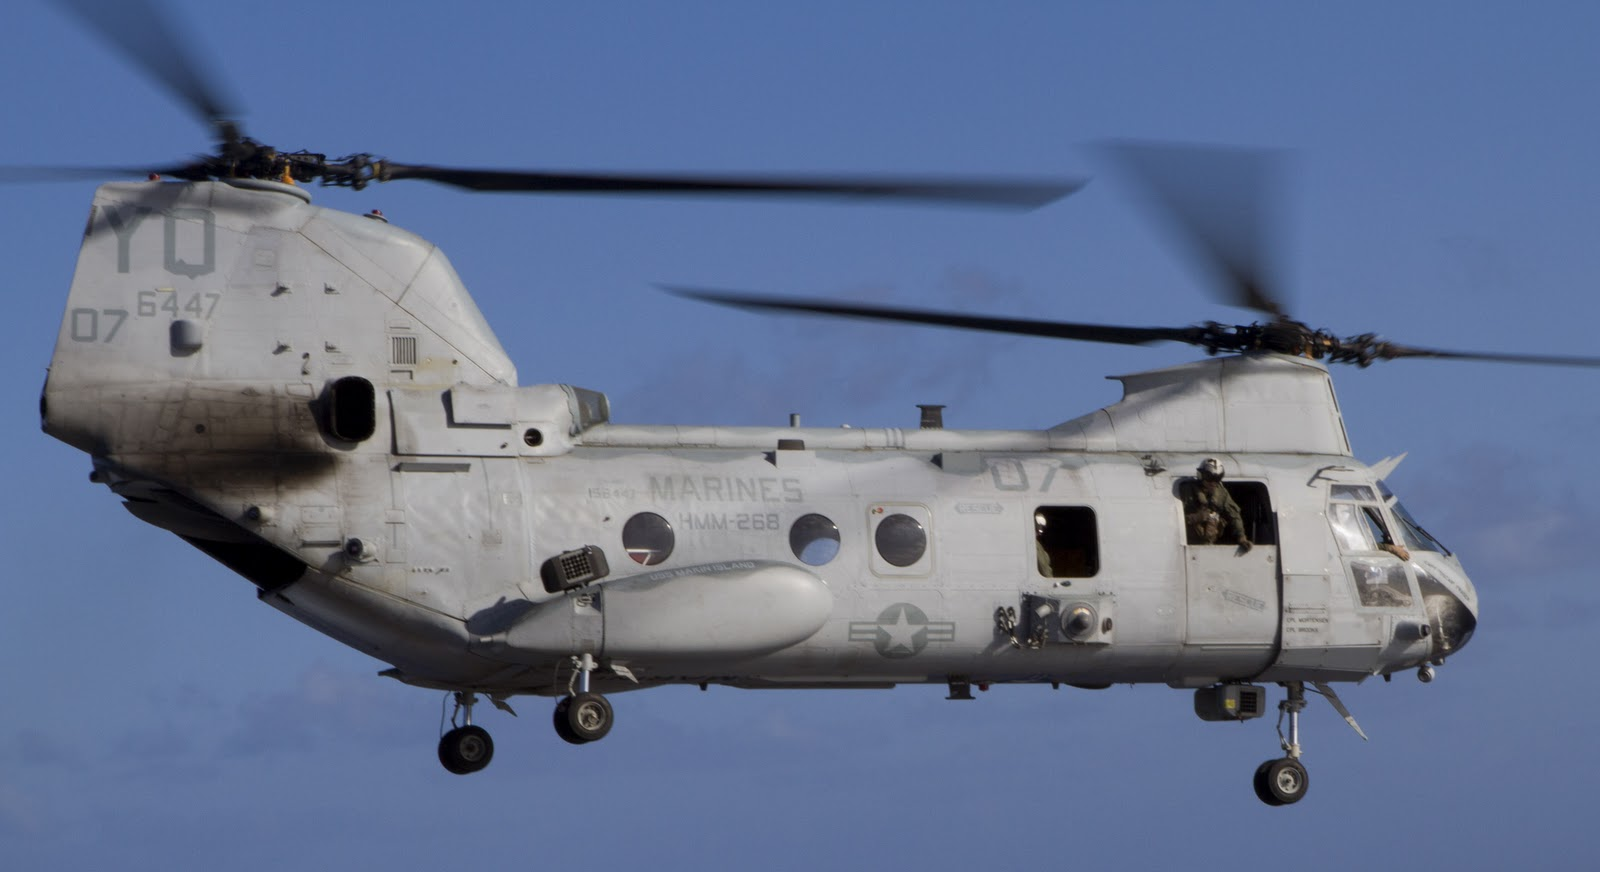
\includegraphics[height = 6cm]{Images/Literature/Tandem}     
	\caption{A military CH-46E Sea Knight, example of a typical tandem rotor}
	\label{IM_Tandem}
\end{figure}


As described in \eqref{EQ_ElectricalPowerThrust} the thrust of the system increases slower than the electrical power input into the system. In a standard configuration, doubling the electrical power would only increase the thrust by a factor of $\approx 1.587$. Where as doubling the amount of rotors being driven will double both the thrust and the electrical power. This gives the tandem arrangement the capability of lifting heavier loads with relatively low power consumption, as well as demonstrating low power consumption for hover and slow translatory flight. Having twin blades does increase the size of the craft, but the elimination of the tail rotor sees the size being similar to that of a classic helicopter.

\subsection{Multirotor Designs}
Drones have joined other remote controlled vehicles in the world of hobbyists. Of all the different designs the multirotor is the most popular. The four rotor design is generally chosen due to its incredible stability and manoeuvrability. Similar to the tandem, quadrotors have very good disk loading and thus can be used to lift heavy loads, there are even products that have 8 rotors to seriously increase the payload capability. This does however relate to a more power hungry system and a less efficient hover.

As shown in Figure \ref{IM_CounterBlades}, a quad rotor consists of two pairs of counter rotating propellers. Each shaft will be driven by its own motor and will contribute to the overall thrust and moment generation of the craft. Having the freedom to control each blade independently gives the pilot advanced manoeuvrability, with minimal mechanical complexities. This also reduces the complexity of the control algorithms as six degrees of freedom can be obtained by simply adjusting the speed of the motors. Besides the poor hover efficiency, the biggest downside of the multirotor designs is their size and weight. Each blade requires a drive system and space to rotate without interference. This generally limits the flight time of multirotors.

\begin{figure}[H]
	\centering
	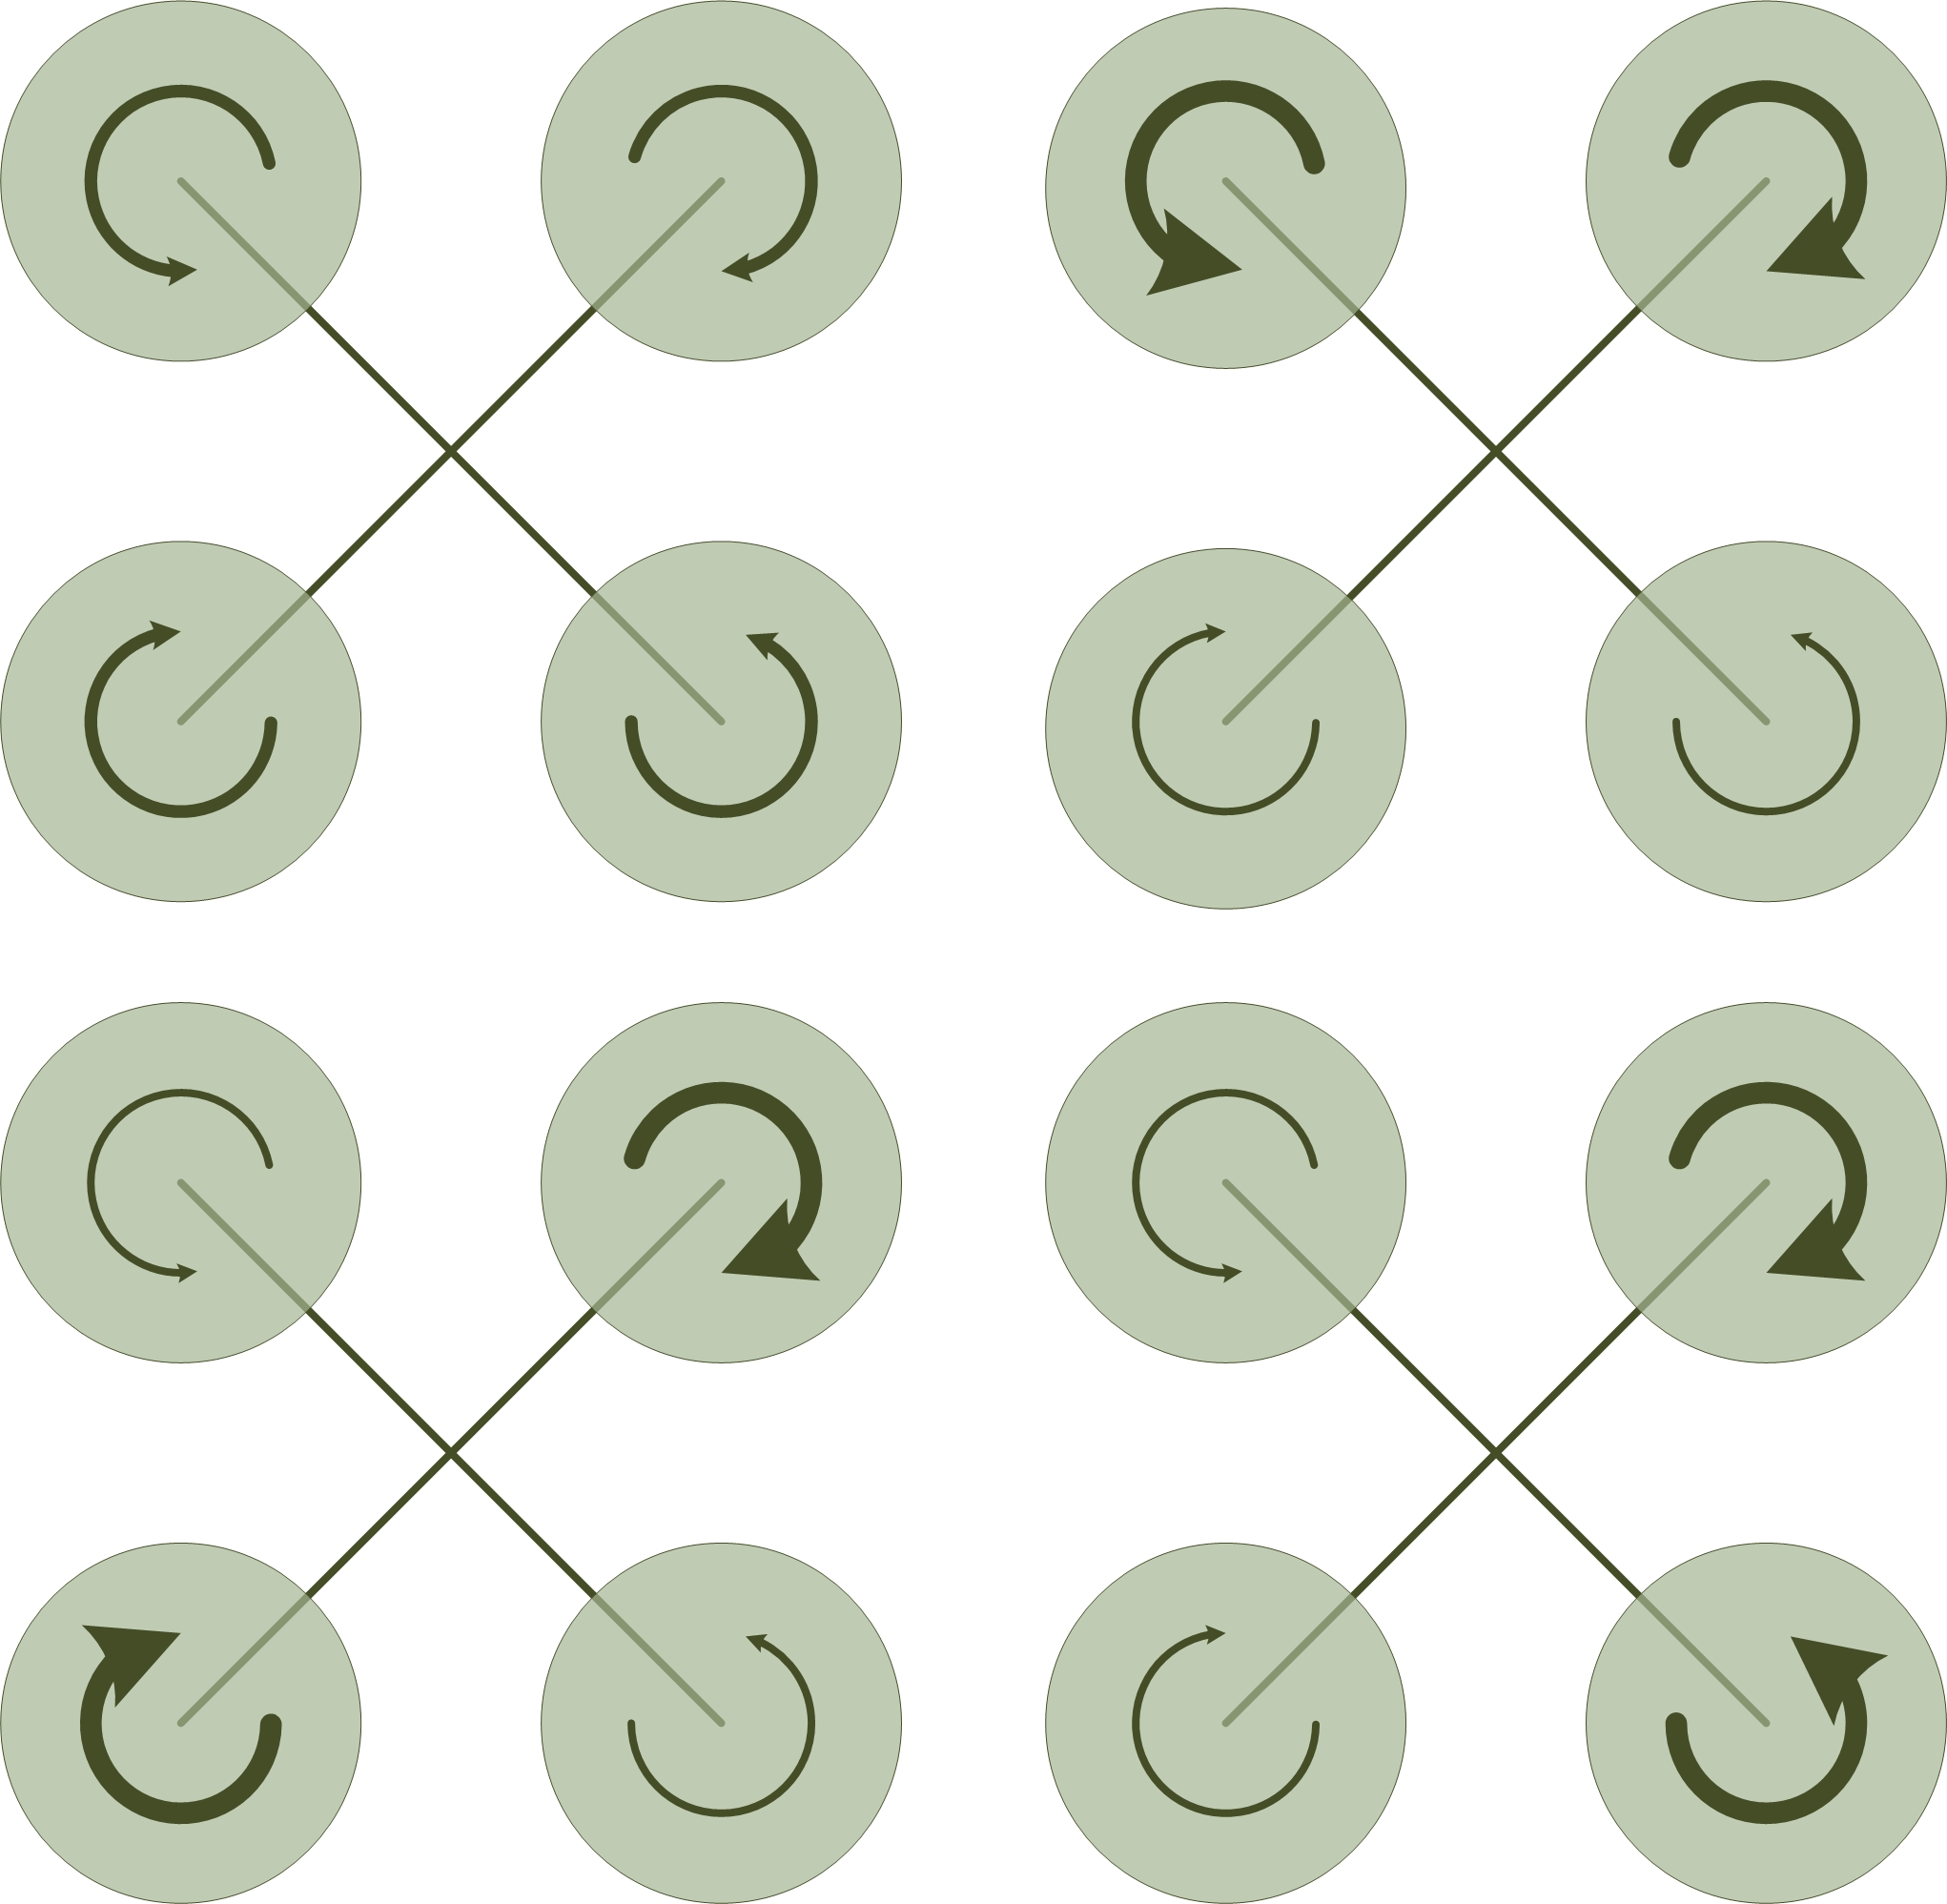
\includegraphics[height =6cm]{Images/Literature/quadrotor}
	\caption{Quadrotor configuration \cite{ThrustCritical}}
	\label{IM_CounterBlades}
\end{figure}

\subsection{Tilt Rotors}
A tilt rotor is a very sophisticated system that attempts to harness the benefits of both the fixed and rotor wing aircraft. With the addition of a pivoting axis for each blade the craft has the forward flying speeds of a fixed wing craft while still being able to take off an land vertically like a rotorcraft. The tilt rotor's major downfall is related to the required highly complex and intricate mechanical design \cite{RotorConfig}.

VTOL applications require a larger blade to decrease the disk loading, while in forward flight a smaller diameter blade is desired to increase the efficiency of propulsion. Hager \cite{US6030177} developed a telescopic system that transforms the blades to get the optimal benefits out of each configuration, shown in figure \ref{IM_TiltRotor}\footnote{(Taken from \cite{Heli})}. These and other improvements have established the tilt rotor as a competitive design in the field of aeronautic transportation \cite{RotorConfig}.

\begin{figure}[H]
	\centering
	\includegraphics[height = 6cm]{Images/Literature/TiltRotor}     
	\caption{Hager's design for a telescopic tilt rotor system \cite{Heli}}
	\label{IM_TiltRotor}
\end{figure}

\subsection{Discussion}


\section{Quadrotor Flight Dynamics}\label{SECT_QuadFlightDynamics}

This section will discuss some of the methods and limitations pertaining to modelling the flight dynamics of a rotorcraft. Most of the discussion will surround multirotors, specifically quadrotors, as the majority of the literature is based on these designs \cite{Luukkonen, RealTime, Pounds2006, Hoffmann, Moller2015}. Due to the mechanical complexity of swashplate designs, the discussion is assuming a fixed pitched rotor set up. 

Before control laws can be applied there must be a dynamic model of the craft. To create the model there must be a good understanding of the factors that effect these dynamics as well as the mathematical methods for deriving the equations. A brief introduction to the nomenclature and axis systems is done and is followed by a discussion into modelling rotorcraft forces and moments. After the model can be obtained mathematically it is important to discuss the physical implementation of obtaining the data, and the instrumentation required. Unfortunately its very rare to have a flying environment that is void of disturbances, this section is closed with a discussion about the various disturbances that effect the flight dynamics of rotorcraft, including some specific environmental disturbances.

	\subsection{Coordinate Systems, Rotations and Nomenclature}
	As the rotorcraft manoeuvres through space, two separate sets of axes are created. Each axis system is important and transforming easily between these frames is necessary. Some of these methods are described in this section, as well as the various means of representing these rotations. This section begins by describing these different frames, namely the inertial and body frames.
		
		\subsubsection{Inertial and Body Frame}
		The inertial, or North East Down (NED), aligns itself with the North and East directions on a compass. The third axis will align with gravity as a positive Z component. This frame assumes that the earth is flat and non-rotating and this frame's origin can be defined arbitrarily.
		
		The body frame aligns itself with the body of the drone, with the nose of the craft facing in the positive X direction and the Z axis is defined perpendicular to the rotor plane with thrust generated in a negative Z direction. The origin of the body frame is defined as the center of mass for the drone.
		
		Figure \ref{IM_Frames} is a visual representation of both frames.
		
		\begin{figure}[H]
			\centering
			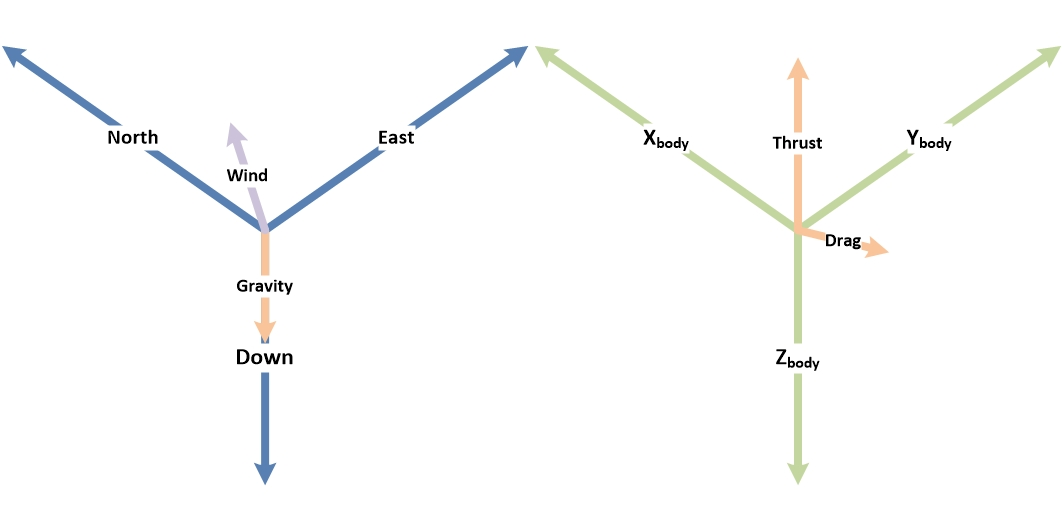
\includegraphics[height = 6cm]{Images/Literature/AxesOverlay.jpg}     
			\caption{The inertial and body frames}
			\label{IM_Frames}
		\end{figure}
			
		In order to relate the motion of the craft in the body frame to the inertial frame, it is necessary to be able to represent the rotation between these frames.
		
		\subsubsection{Euler Angles}	
		The most intuitive way to represent the rotation between two frames, is by looking at the rotation between each corresponding axis. These are known as the Euler angles and are made up of a roll ($\phi$), pitch ($\theta$) and yaw ($\psi$) angles. Euler angles provide a very intuitive understanding of the rotation between the different frames. This is best explained with Figure \ref{IM_Euler}.
		
		\begin{figure}[H]
			\centering
			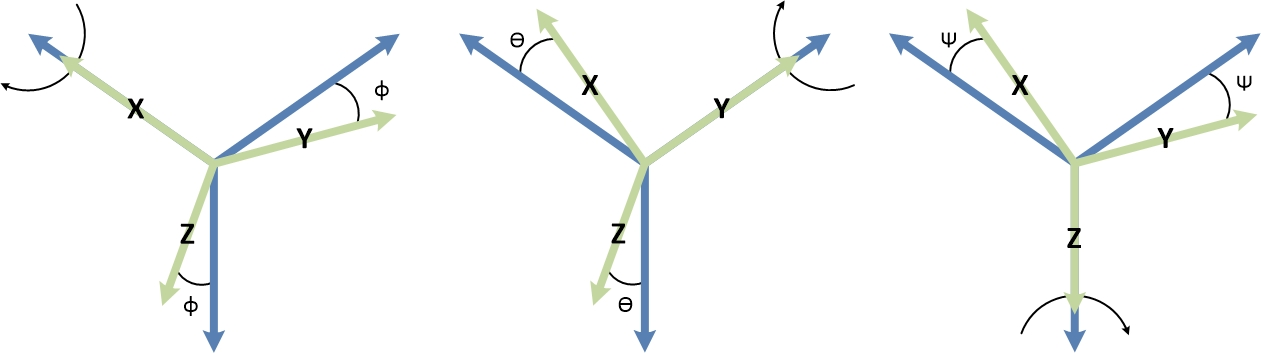
\includegraphics[height = 4cm]{Images/Literature/rotations.jpg}     
			\caption{Individual rotations around the X, Y and Z axes respectively.}
			\label{IM_Euler}
		\end{figure}
		
		The yaw angle is defined as a pure rotation around the Z-Axis. Roll and pitch are defined as pure rotations around the X-Axis and Y-Axis respectively. The Euler angle representation does have limitations, such that any 3 Euler angles could represent a different rotation, based on the order it is applied. For this project, a Euler 3-2-1 sequence will be followed. There is also a chance of a singularity at extreme angles, this is not a concern for this project, as it will only be necessary to ever complete small rotations \cite{quaternion, Moller2015}. 
		
		According to Euler's theory, any two varying coordinate axes can always be related to one another by a single rotation. 
			
		\subsubsection{Direct Cosine Matrix}
		The direct cosine matrix (DCM), provides a simple method for transforming references between two different frames. This is necessary for converting the NED frame to the body frame and vice versa. The DCM is calculated by following 3 individual rotations and multiplying their results together. A 3-2-1 Euler sequence will transform first using yaw then pitch and finally roll. Each transformation is represented as a 3x3 Matrix representing a rotation around one of the axes.
		
		In the case of rotating from the body to the NED frame, the matrix takes the form as shown in equation \eqref{EQ_RotationMatrix} \cite{Luukkonen, Moller2015} where $C_x = \cos(x)$ and $S_x = \sin(x)$. The matrix is also orthogonal, which means that $\textbf{R}^{-1} = \textbf{R}^T$. $\textbf{R}^T$ would be the rotation from the inertial frame to the body frame \cite{Luukkonen, Moller2015, quaternion}.
		
		\begin{equation}
		\label{EQ_RotationMatrix}
		\textbf{R} = 
		\begin{bmatrix}
		C_\psi C_\theta   	& C_\psi S_\theta S_\phi - S_\psi C_\phi & C_\psi S_\theta C_\phi + S_\psi S_\phi \\
		S_\psi C_\theta   	& S_\psi S_\theta S_\phi + C_\psi C_\phi & S_\psi S_\theta C_\phi - C_\psi S_\phi\\
		-S_\theta   		& C_\theta S_\phi & C_\theta C_\phi  \\
		\end{bmatrix}
		\end{equation}
		
		The DCM does provide a mathematically simple method for creating relationships between frames, however this method is computationally taxing as it is forced to recalculate the matrix and the multiplications on every loop.
		
		\subsubsection{Quaternions}
		The quaternion representation manages to minimise the computation required to calculate transformations, as well as remove the singularity found in the Euler representation \cite{quaternion}. One of the major downsides of quaternions is that they are difficult to interpret intuitively. A quaternion follows the form seen in \eqref{EQ_Quaternion} and contains a scalar value $q_w$ and a vector component $[q_x \ q_y \ q_z]$. This representation is broken up into a rotation angle, and a rotation axis.
		
		\begin{equation}
		\label{EQ_Quaternion}
		\textbf{q} = 
		\begin{bmatrix}
		q_w \\
		q_x\\
		q_y\\
		q_z\\
		\end{bmatrix}
		\end{equation}
		
		Quaternions come with their own set of mathematical rules and laws which will not discussed here. However it should noted that their are techniques that provide simple conversion from and to Euler angles and thus the DCM.  
		
		\subsubsection{Nomenclature}
		The naming convention used, follows Moller's notation \cite{Moller2015} and is shown in \ref{TAB_Nomenclature}. It makes sense that the global position and velocity of the craft be described in the NED frame, however the forces and moments will be generated in the body frame. Since there is now a simple relationship between the two frames, it is possible to relate the body frame forces and movements, into earth frame translations. The variables shown in Table \ref{TAB_Nomenclature} are visualised in Figure \ref{IM_Nomenclature}. The variables are all defined in the body frame and are shown, along with their positive directions. The right hand and thumb rule were used to dictate direction.
		
		\begin{figure}[H]
			\centering
			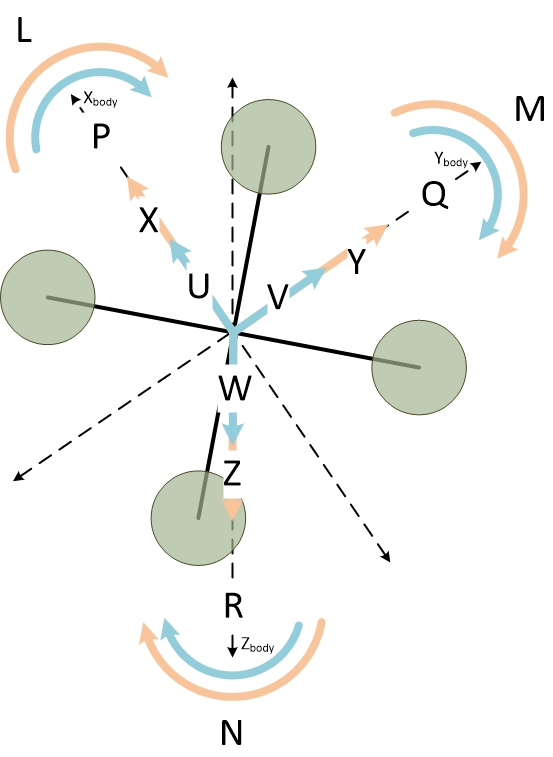
\includegraphics[height = 10cm]{Images/Literature/ForcesMoments.jpg}     
			\caption{Typical naming convention of body forces, moments and velocities for a quadrotor}
			\label{IM_Nomenclature}
		\end{figure}
		
		\begin{table}[!]
			\centering
			\begin{tabular}{| l | l |}
				X, Y, Z 	& Force vector along the respective body frame axis\\
				L, M, N 	& Moment around the respective body frame axis\\
				U, V, W 	& Linear velocity along each body frame axis\\
				P, Q, R  	& Angular velocity around each body frame axis\\
			\end{tabular}
			\label{TAB_Nomenclature}
			\caption{Standard Nomenclature}
		\end{table}
		
		The body frame forces, moments and velocities can be seen, and are described in \eqref{EQ_ForcesMomentsVelocitiesX} - \eqref{EQ_ForcesMomentsVelocitiesN}. Where X, Y, Z are the forces in each body axis, with the rotor thrust being produced in the negative Z direction. L, M, N are the moments around the x, y, z axes respectively and U, V, W are the velocities aligned with the x, y, z axes respectively. 
		
		Using the rotation matrix described in \eqref{EQ_RotationMatrix}, a relationship for North, East and Down velocities can be made and is described in \eqref{EQ_UVWtoNED}. 
		
		\begin{equation}
		\begin{bmatrix} \dot{N}\\ \dot{E}\\ \dot{D} \end{bmatrix} = \textbf{R} \begin{bmatrix} U\\ V\\ W \end{bmatrix}
		\label{EQ_UVWtoNED}
		\end{equation}
				
	\subsection{Kinetics and Kinematics}
	
	Assuming the system can be considered as a rigid body, allows for the use of normal Newtonian mechanics to create the equations of motion. This method will also use the Euler angles described above \cite{Luukkonen, Modelling, Moller2015}.
	
	The derivations of these calculations are well documented in literature \cite{Blakelock}
	
	\begin{eqnarray}
	X &=&  m(\dot{U} - VR + WQ)\label{EQ_ForcesMomentsVelocitiesX}\\
	Y &=&  m(\dot{V} - UR + WP)\label{EQ_ForcesMomentsVelocitiesY}\\	
	Z &=&  m(\dot{Q} - UQ + VP)\label{EQ_ForcesMomentsVelocitiesZ}\\
	L &=&  \dot{P}I_{xx} + QR(I_{zz} - I_{yy})\label{EQ_ForcesMomentsVelocitiesL}\\
	M &=&  \dot{Q}I_{yy} + PR(I_{xx} - I_{zz})\label{EQ_ForcesMomentsVelocitiesM}\\	
	N &=&  \dot{R}I_{zz} + PQ(I_{yy} - I_{xx})\label{EQ_ForcesMomentsVelocitiesN}
	\end{eqnarray}
	
	
	\subsection{Mass Model and the Inertia Tensor}
		\subsubsection{Mass Model}
		In any aerial vehicle mass is always an important design criterion. Every aspect of the platform must be designed to be the lightest it possibly can. Having a light weight craft is one part of the design criterion, another would be ensuring that the weight is geometrically spread out correctly, as well as functionally distributed appropriately. The table below was adapted from \cite{NewMAV} and demonstrates the latter point by showing the weight distribution of three separate crafts. Depending on the different criteria for the craft, different functional blocks will be allocated a certain percentage of weight. For example if the project requires a longer flight time, a higher percentage would be given to the power source and possibly less to the external payload. Generating a good mass model before designing helps better understand the requirements for the craft and could be a deciding factor in the construction.
		
		\begin{table}[H]
			\centering
			\begin{tabular}{l | c | c | c | c}
				
				Component 					& 0.3kg & 1.8kg & 3.7kg\\
				\hline\hline
				Rotor System 				& 11.0 & 11.2 & 13.9\\
				Tailboom Assembly 			& 8.0 & 9.1 & 7.8\\
				Main Rotor Motor 			& 15.4 & 10.5 & 8.1\\
				Fuselage/Structure 			& 7.0 &  15.1 & 12.0\\
				Main Transmission 			& 2.0 &  3.4 & 3.4\\
				Landing Gear 				& 2.3 &  3.4 & 2.9\\
				Control System 				& 5.7 & 18.3 & 9.3\\
				Avionics 						& 29.4 &  2.4 & 1.6\\
				Power Source 				& 19.2 & 26.6 & 41.0\\
				
			\end{tabular}
			\caption{MAV Weight Data (Adapted from \cite{NewMAV})}
		\end{table}
	
		\subsubsection{Inertia Tensor}
		It was also mentioned that the weight needs to be geometrically positioned correctly, the point of this would be to create as much symmetry in the craft as possible. If this is done correctly the principle axes of inertia will align very closely with the body of the craft, simplifying calculations later on and helping find and define the principle axes. The inertia tensor is a matrix that is a representation of a rigid body's resistance to rotations in 3D space. For the general case the inertia tensor takes the form as shown in equation \eqref{EQ_InertiaTensor}. The inertia tensor is very dependant on a craft's symmetry, and is symmetric itself. In other words, $I_{xy} = I_{yx}$, $I_{xz} = I_{zx}$ and $I_{zy} = I_{yz}$ and therefore if a craft is symmetric about the X, Y and Z axes, then the assumption can be made that $I_{xy} = I_{yx} = I_{xz} = I_{zx} = I_{yz} = I_{zy} = 0$ \cite{Luukkonen, MiniFlying}.
		
		\begin{equation}
		\label{EQ_InertiaTensor}
		\textbf{I} = 
		\begin{bmatrix}
		I_{xx}	& -I_{xy} & -I_{xz}\\
		-I_{yx}	& I_{yy}	& -I_{yz}\\
		-I_{zx}	& -I_{zy}	& I_{zz}\\
		\end{bmatrix}
		\end{equation}
		
		In order to successfully model a rotorcraft, the inertia tensor must be known and will be defined around the centre of rotation of that rotorcraft. The method for obtaining the inertia tensor is described in the system identification of this project.
		
	\subsection{Rotor Generated Forces and Moments}\label{SSECT_RotorForcesMoments}
	The forces and moments generated by the rotors are discussed here. It is assumed that the rotors will only generate a force perpendicular to their plane while the moments are dependant on the placement of the rotors.
	
	\begin{figure}[H]
		\centering
		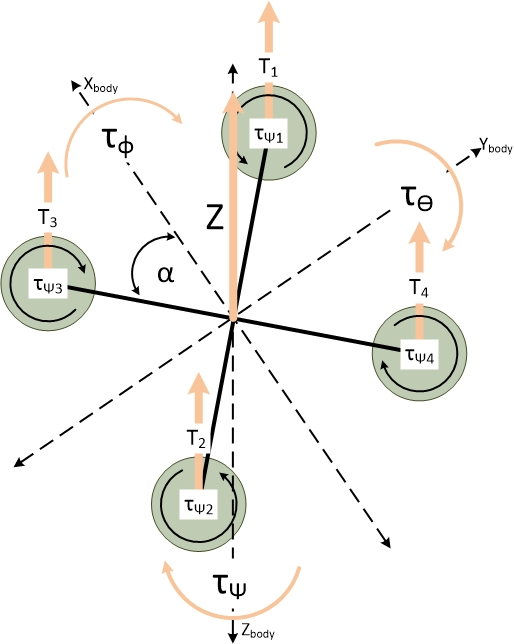
\includegraphics[height = 10cm]{Images/Literature/quadforces.jpg}     
		\caption{Forces and moments acting in the body frame on an X-Configuration quadrotor}
		\label{IM_Forces}
	\end{figure}
	
	
		\subsubsection{Actuators}
		As shown in Figure \ref{IM_Forces}, all the forces generated by the quadcopter are a product of the four rotors. The rotors convert mechanical energy from the motors into aerodynamic power. The motors convert electrical energy into mechanical energy based on the motor commands sent from the controller. Both the motors and rotors can not react instantly to new commands, this lag introduces a timing delay constant into the system \cite{Moller2015}.
		
		If the lag timing constant is defined as $\tau$, thrust generated by motor $x$ as $T_x$ and the command sent to that motor as $T_{xR}$. Then \eqref{EQ_MotorDelay} can be created and applies to all four motors.
		
		\begin{equation}
		T_x = -\dot{T_x} \tau + T_{xR}
		\label{EQ_MotorDelay}
		\end{equation}
		 		
		\subsubsection{Controlled Body Forces}
		Figure \ref{IM_Forces} assumes that all of the rotors lie in the same plane, and only provide a unidirectional force. This assumption allows the easy creation of a total force $\textbf{T}$, which is shown in \eqref{EQ_Translational} as the sum of all four motor thrusts. 
		
		\begin{eqnarray}
		Z = (T_1 + T_2 + T_3 + T_4)
		\label{EQ_Translational}
		\end{eqnarray}
		
		To command this value, a virtual actuator can be created $\delta_{Z}$ which commands all four rotor thrusts. Equation \eqref{EQ_MotorDelay} demonstrates the lag to generate these thrusts and the same lag dynamics will apply to $\delta_{Z}$, thus creating \eqref{EQ_VirtualHeave}.
		
		\begin{eqnarray}
		Z = -\dot{Z} \tau + \delta_Z
		\label{EQ_VirtualHeave}
		\end{eqnarray}
				
		\subsubsection{Controlled Body Moments}
		A quadrotor generates a moment around it's own axis through varying the speed of each motor. The torque generated is also dependant on the spacing for the type of quadrotor used. A standard X-Configuration quadrotor is shown in Figure \ref{IM_Forces} and was used for this analysis. To induce a torque around the X-axis, the sum of the two left rotors subtracted from the sum of the two right rotors must be non-zero. Similarly the front and back rotor summations must not be equal to induce a torque around the Y-axis. As shown in \ref{IM_Forces}, each rotor also creates a moment around the Z-axis. This induced torque is a product of the rotors lift to drag ratio and the chord length and is represented in \eqref{EQ_YawTorque}.
		
		\begin{equation}
		\tau_{\psi x} = \frac{r_D}{R_{LD}} \times T_x
		\label{EQ_YawTorque}
		\end{equation}
				
		Assuming that each rotor has the same characteristics and are spaced evenly, these moments can be mathematically expressed as shown in \eqref{EQ_Torques}, where $l$ is the distance from the centre of the rotor to the centre of gravity, $r_D$ is the chord length and $R_{LD}$ is the lift to drag ratio for the rotors.
				
		\begin{eqnarray}
		L &=& \frac{r_D}{R_{LD}} \times (T_3 + T_4 - T_1 - T_2)\\
		M &=& (T_1 + T_3 - T_4 - T2) \times lcos(\alpha)\\
		N &=& (T_2 + T_3 - T_1 - T4) \times lsin(\alpha)
		\label{EQ_Torques}
		\end{eqnarray}
		
		Virtual actuators can be created to command these moments, namely $\delta_\psi$, $\delta_\theta$ and $\delta_\phi$. However these commands will be subject to the same time delay experienced by the rotors. Therefore \eqref{EQ_VirtualTorquesL} - \eqref{EQ_VirtualTorquesN} can be used to represent the relationship between these commanded values and the actual moment \cite{Modelling, Moller2015}.
			
		\begin{eqnarray}
		L &=& -\dot{L} \tau + \delta_\psi\\ \label{EQ_VirtualTorquesL}
		M &=& -\dot{M} \tau + \delta_\theta\\ \label{EQ_VirtualTorquesM}
		N &=& -\dot{N} \tau + \delta_\phi \label{EQ_VirtualTorquesN}
		\end{eqnarray}
				
	
	\subsection{Disturbances}\label{SSECT_Disturbances}
	
		\subsubsection{Drag}\label{SSSECT_Drag}
		Drag is a damping force whose quantity is relative to the speed of the object, and always opposes the direction of motion. Drag is defined here in the body frame and from \eqref{EQ_Drag} and the discussion drag, the equations for three dimensional drag can be calculated. As shown in \eqref{EQ_dragForcesX} - \eqref{EQ_dragForcesZ}, the effect of drag can be reduced through mechanical design and flight strategy, by reducing the area of the plane facing towards the direction of the motion. 
		
		\begin{eqnarray}
		F_{Dx} &=& C_{DX} (\dfrac{1}{2} \rho U^2) A_{YZ} \label{EQ_dragForcesX}\\
		F_{Dy} &=& C_{DY} (\dfrac{1}{2} \rho V^2) A_{XZ} \label{EQ_dragForcesY}\\
		F_{Dz} &=& C_{DZ} (\dfrac{1}{2} \rho W^2) A_{XY} \label{EQ_dragForcesZ}
		\end{eqnarray}
		
		Due to an offset between the centre of gravity and the centre of pressure, the drag forces can also create undesired moments. Equations \eqref{EQ_dragMomentsL} - \eqref{EQ_dragMomentsL} can be derived from the Figure \ref{IM_dragForces}, where $d_x, d_y, d_z$ are the offsets of the centre of pressure. $F_{Dx}, F_{Dy}, F_{Dz}$ are the forces generated by drag act along the coinciding body axis. $M_{Dx}, M_{Dy}, M_{Dz}$ are the and moments generated by the drag forces and the offset of the centre of pressure, they act around the coinciding axis. $A_{YZ}, A_{XZ}, A_{XY}$ are the surface areas facing the corresponding plane in the body frame with $C_{DX}, C_{DY}, C_{DZ}$ as the corresponding drag coefficients.
		
		\begin{eqnarray}
		M_{Dx} = F_{Dz} \times d_y - F_{Dy} \times d_z \label{EQ_dragMomentsL}\\
		M_{Dy} = F_{Dx} \times d_z - F_{Dz} \times d_x \label{EQ_dragMomentsM}\\
		M_{Dz} = F_{Dy} \times d_x - F_{Dx} \times d_y \label{EQ_dragMomentsN}
		\end{eqnarray}
		
		\begin{figure}[H]
			\centering
			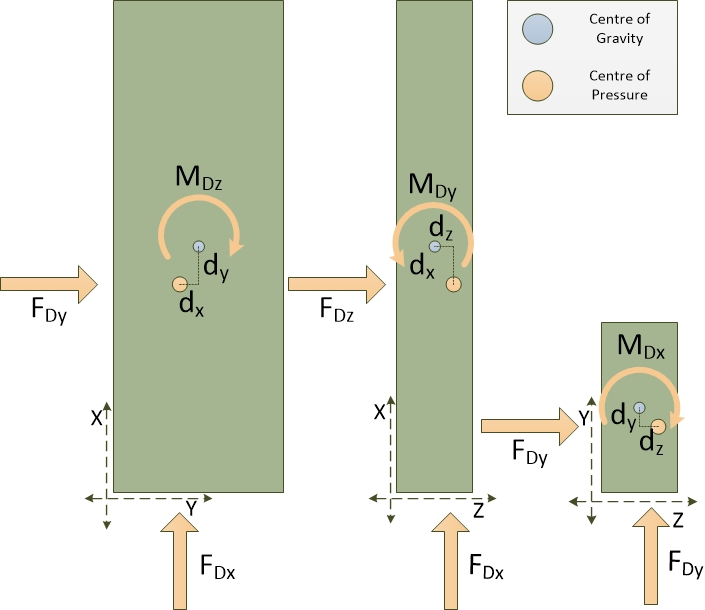
\includegraphics[height = 8cm]{Images/Literature/drag.jpg}     
			\caption{Typical moments created by drag forces}
			\label{IM_dragForces}
		\end{figure} 
				
		\subsubsection{Airflow Characteristics}
		
		In the preceding section on flight theory, the importance of air density, pressure and the creation of rotor wake boundary are discussed. The negative effects of disrupting airflow as well as the need for controlling this disturbance has been well documented in literature \cite{NearWall, Lee2012, Hoffmann}.
		
		Using Figures \ref{IM_MomentumTheoryAirFlow} and \ref{IM_MomentumTheoryHover} as references Airflow can be seen as the stream of air from $v_0$ to $v_\infty$\, through $v_i$. Equation \ref{EQ_ThrustMass} states that thrust is directly proportional to the relationship between these velocities and any deviation in these velocities will vary the thrust of the rotor in question. $v_0$ is only zero when the craft is in a state of pure hover, completely stationary, and there is no wind. Increasing the speed of the craft will increase the $v_0$ component creating a variation in the overall thrust, the same can be said for any condition that contains a tangible wind factor. 
		
		As investigated by \cite{Hoffmann} mechanical intrusions will have an effect on the far wake velocity, thus also effecting the generated thrust. In the design of STARMAC by Hoffmann et al \cite{Hoffmann} the frame was designed to be very configurable so that the effects of the mechanical design could be quantified. Originally the rotors were shrouded and quite close to the centre of gravity of the craft. The shrouds were a distance of 5\% rotor radius and when removed the yaw tracking improved from $\pm$10\textdegree to $\pm$3\textdegree. When not included in the dynamic model the obstruction in the air stream will cause lower and less stable values of thrust, affecting the accuracy of the model. 
		
		When the rotors were located close to the centre of gravity they obtained some attitude disturbances that were eliminated by moving the rotors further away. It was also observed that any object that lies close to the rotor tip, created intense arbitrary disturbances and should be avoided \cite{Hoffmann}.
		
		\cite{NearWall} attempts to model some of the disturbances for a single rotor craft hovering near wall, but as stated by \cite{Lee2012} it is not viable to accurately quantify these disturbances, however their presence must not be neglected. As Figure \ref{IM_NearWallF} shows, these can be modelled as a disturbance to the input force and moments.
		
		\begin{figure}[H]
			\centering
			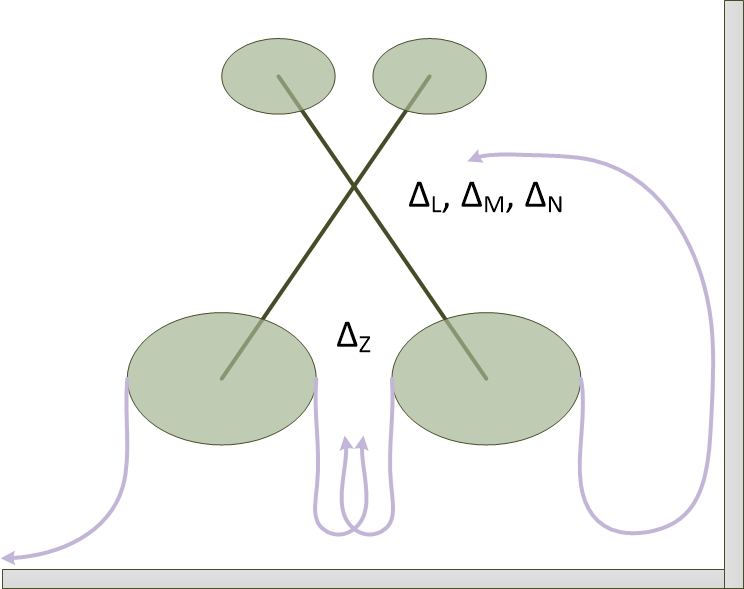
\includegraphics[height = 7cm]{Images/Literature/near_wall}     
			\caption{Velocity components though the rotor for, no wall (left) and near wall (right) conditions (Taken from \cite{NearWall})}
			\label{IM_NearWallF}
		\end{figure}
		
		As demonstrated by \cite{NearWall}, there is also an induced moment acting on the rotor as the rotor approaches the wall. Figure \ref{IM_NearWall} is an image generated by \cite{NearWall}, it demonstrates the change in airflow on a rotor close to a wall region.
		
		\begin{figure}[H]
			\centering
			\includegraphics[height = 5cm]{Images/Literature/NearWall}     
			\caption{Velocity components though the rotor for, no wall (left) and near wall (right) conditions (Taken from \cite{NearWall})}
			\label{IM_NearWall}
		\end{figure}
		
		In \cite{NearWall}, Robinson et al used the script $c$ as their unit of measure for distance to the wall, $c$ is chord length of the airfoil. The graph shown in Figure \ref{IM_NearWallGraph} shows how the moment felt by the craft varies with the distance to the wall. The direction of the moment will be perpendicular to the wall. As above, this disturbance can also be modelled as a variation to the input moments to the system.
		
		\begin{figure}[H]
			\centering
			\includegraphics[height = 5cm]{Images/Literature/NearWallGraph}     
			\caption{Graph showing relationship between distance from the wall and moment felt be the craft (Taken from \cite{NearWall})}
			\label{IM_NearWallGraph}
		\end{figure}
		
		In \cite{NearWall} they conclude their paper by describing a proposed method of control which will be investigated further in this text. This dynamic flight model requires sensing of specific craft variables, typical sensing methods and requirements are discussed in the proceeding section. 
	
	\subsection{Instrumentation}
	The need for a well instrumented craft is intuitive and well documented in literature \cite{Moller2015, Hoffmann}. With modern advancements in sensing technology there is now a number of methods to obtain the required information. However, some of these are very costly and require specific operational environments. For this purpose, only the inertial measurement unit (IMU) and the global positioning system (GPS) are discussed here.
	
		\subsubsection{Inertial Measurement Unit}
		Traditionaly an IMU will consist of an accelerometer, gyroscope and possibly a magnetometer. The accelerometer has the ability to measure accelerations in the body axis. It should be noted that an accelerometer in rest, sitting along the inertial axis will provide a reading of $[0\  0\  g]^T$. The gyroscope measures the rotational accelerations of the craft, thus measuring 6 degrees of freedom in total. Unfortunately gyroscopes suffer from sensor drift and needs compensation. The accelerometer's gravity offset can be used to align with the vertical axis, however a magnetometer is required to account for drift in the horizontal plane. Various filtering and fusion techniques are used to combine these readings, the most popular of which  is a Kalman Filter \cite{Moller2015, Hoffmann}.
		
		\subsubsection{Global Positioning System}
		The most common method of measuring a drone's position is with the use of a GPS. The GPS readings can also be used to create an estimate of the craft's linear velocity in the inertial frame. When combined, multiple GPS unit's can be used to obtain higher precision. A major downside of a GPS is the dependence on a satellite link, this dependence severely limits the operational environments for this sensor. Other methods of localisation include using known maps and proximity sensing to provide the rotorcraft with position estimates. As discussed, these techniques are out of scope for this project and will not be considered. This project will assume an earth position and velocity estimate are present, subject to filtered noise provided through band limited white noise \cite{Moller2015}
		
		\subsubsection{Measurement Noise}
		From the discussion it is evident that sensors will not be without error. The noise associated with the measurements will be different for both varying sensor types and manufacturers and will depend on the chosen sensors. The characterisation of the noise for this project is discussed in the system identification chapter. The environment in which these sensors operate also has a significant effect on operation. Moller characterises this measurement noise as a random band limited white noise block. and adds a low pass filter to the GPS measurements \cite{Moller2015}.

\section{Collision Protection Techniques}
	Collision protection is an addition to any platform that will assist under during an impact. An advanced enough collision protection technique could negate the risk of impact in a confined environment. Any obstruction in a rotor's path will either destry the part, or stop it from spinning thus disabling the thrust generation capacity of that rotor. Collision protection in it's simplest form is a simple shroud that can protect the rotors. 
	
	\subsection{Impact Resistance}
	Impact resistance is a technique used by a variety of fields in the world today. Included in this is something as simple as the shocks or suspension in a car, they are designed to allow the automotive to withstand sudden impacts. Generally these techniques use a component that has some tangible spring constant that can be sued to absorb the energy felt during an impact.
	
	Klaptocz et al investigated such a system for an aerial vehicle \cite{Klaptocz2013}. Using a combination of drop tests and forced collisions it was validated that an impact resistance shroud could limit the force felt by the platform. Light weight materials can be used to create the design however there inevitably will be additional weight and size added to the platform.
	
	\subsection{Rolling Cage}
	Although impact resistance can limit the effect of a collision Briod et al set out to create a system truly robust to collisions \cite{Collision, Briod2012, Klaptocz2010}. Using a coaxial rotorcraft they developed a system whereby, using a three axis gimbal, an external shell will passively rotate around the craft on impact. Thus almost negating the effect of the collision completely. Although a proven solution to confined indoor flight, the system is optimised for a coaxial rotorcraft limiting the payload and flight time capabilities of the design.  
	
\section{Review of Existing Flight Control Strategies}\label{SECT_ControlReview}
The object of this section is gain a better of understanding of successful controller designs and implementations. A talented pilot could fly a rotorcraft with minimal assistance from an on board controller, however to successfully create an autonomous vehicle capable of flight in a confined environment, a robust controller design is required. The discussion is broken into two sections, first a look into high level controller architectures is done after which a look into some successful real world implementations is investigated. The different axis systems used are discussed in a previous section and transition between these axes becomes a crucial part of the controller architecture.

	\subsection{Controller Architecture}
	Traditional tracking control for a rotorcraft is distributed between three controllers, namely an altitude, heading and horizontal controller \cite{Moller2015, Mellinger2014}. The specific loop structure is determined by which feedback is available to close the loops. These loops are made up of combinations of traditional control laws such as PID controllers and Lead-Lag compensators.
	
	The altitude controller is straight forward, dynamics are derived directly from Newton mechanics. A traditional structure is the use of three cascaded loops. The most inner loop can control the linear acceleration of the craft in the body frame and it's loop can be closed by use of an accelerometer. The next loop is used to control the climb rate of the craft in the earth frame, with the final loop controlling the final position of the craft. The altitude loop is closed by some form of altimeter, traditionally a barometer can be used to estimate altitude. For more precise altitude control a sensor can be used to give a relative height above the ground. The velocity loop is generally closed by some approximation of velocity through differentiation of absolute position. In some cases optical flow sensors could be used to obtain a velocity measurement directly.
	
	The heading controller is responsible for controlling the orientation of the craft. Traditional quadcopters can fly omni-directionally irrespective of their heading, allowing for less stringent design requirements on this controller. Orientation is traditionally described as a Euler angle off of a given axis obscuring the axis systems and need for rotations. The heading controller can be simply broken into two loops, an inner rate loop and an outer angle loop. Both of which can be closed by the use of an IMU combining magnetometers and gyroscopes.
	
	The final and most complex controller structure is the horizontal control. This is the only controller that is required to control both angular and translational control loops introducing the need for inferring desired angles from a given translational reference. The controller generally is also required to work in both axis systems, requiring some form of geometric transformation. The translational portion of the controller is split up into a North and East controllers, while the inner angular system is broken up into roll and pitch controllers. The translational portion is further broken down into an outer position loop which feeds setpoints to an inner linear velocity loop. Both of these loops can be closed by a GPS unit. The angular portion of the controller is then also split into a inner rate loop which is potentially closed by a gyroscope and an angular position loop which utilises feedback from an IMU.
	
	Tracking control is used to obtain stable flight and reject disturbances and unmodelled errors. However certain disturbances might hinder the performance of these controllers and produce instability that traditional control law can not account for without negatively affecting the tracking control. Feed forward control could be utilised if the disturbances can be predicted and their effects have been quantified, this however is rarely the case.   
	
			\subsubsection{Disturbance Based Observer Controller}\label{SectionDisturbanceObserver}
			Another method of rejecting extreme disturbances, while limiting the adverse effects on the tracking control, is to estimate the disturbance and then control based on that estimation. In an investigation of the near wall effects, Robinson et al propose a disturbance based observer which can be used to predict and counteract these disturbances \cite{NearWall, Robinson2016}. Figure \ref{IM_DOBC} outlies the structure of such a controller, and demonstrates how it is interfaced with traditional tracking control. The main benefit of this structure is the loop is only activated when the state estimations do not match the state outputs. 
			
			\begin{figure}[H]
				\centering
				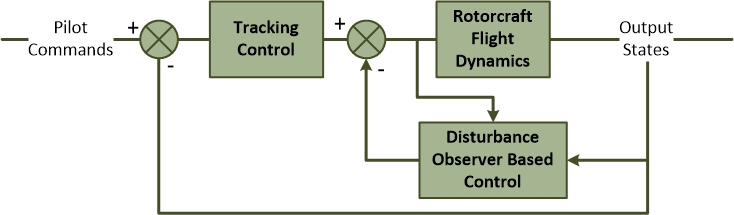
\includegraphics[height = 4.5cm]{../References/Diagrams/DOBC}     
				\caption{Disturbance Observer Based Controller Structure}
				\label{IM_DOBC}
			\end{figure}
			
			For a system like this to be effective, the observer will need to measure the disturbances in real time requiring fast computation. Lee et al implemented an adaptive control strategy which uses an IMU and a Vicon system to estimate the disturbances and feeds them into the system \cite{Lee2012}. This requires a complex lab set up and can not be used in any environment, however their experiments did validate the effectiveness of such a system.

	\subsection{Controller Implementation}
	Controller design and controller implentation vary 
	
	The open source software framework, ArduPilot is a well developed code base. The quadrotor code was also reviewed to establish an understanding of implementing these 
	\cite{Meier2015}
	

	
	
\section{Collision Avoidance Techniques}
Some protection techniques were described above to assist the craft in the event of a collision. However, these techniques add weight, complexity and in some instances obstruct potential sensors. Near wall disturbances have also been discussed and can severely impact a rotor craft flying in a confined space. Using the more simple protection techniques, it is still desirable to avoid collisions all together. Collision and obstacle avoidance sensing techniques can also be used to aid in a higher route planning algorithms. For successful collision avoidance, the craft must be able to collect data about it's surroundings. This section begins by describing some of these sensing techniques and finishes by investigating some of the methods for utilising this data.

	\subsection{Sensing Techniques and Requirements}
	Traditionally the collision avoidance sensing techniques can be broken into two main categories. Namely some form of proximity measurement can be done, or a higher level more intelligent image processing system can be applied \cite{Green2015}. This discussion analyses each of these hierarchies separately.
	
		\subsubsection{Proximity Measurement}		
		The first and most common would be using a time of flight (TOF) sensor, such as an ultrasonic transducer. Very similar to bats, a transmitter module will emit a pulse and based on the time it takes for the signal to return, the distance can accurately be measured. A sonar is dependant on a lot of variables and would require calibration for the environment it is in. Due to the method with which the modules acquire information the drone will be receive a speed limitation. Since the sonar is dependant on the density of the medium it travels through, disturbance created by the rotors could severely affect the performance of the sensors.
		
		Another option in the same category would be to use an infra red (IR) transceiver in the same configuration. The system uses strobed IR pulses to monitor the distance of an object, the system depends on the ratio of reflection for the IR spectrum. If an object as a high refraction or absorption ratio the signal can get lost. Ambient light can also cause interference, although most modules will have some form of built in filter. Both these methods are also sensitive to the angle at which they are measuring. 
		
		Using the same base technology TOF cameras have been developed such as Microsoft's Kinect. Instead of a single point, a TOF camera projects an IR grid into the area it wishes to explore. By measuring deviations in the expected grid structure, distance information can be inferred. In an IR rich environment, TOF cameras can get overwhelmed and produce unreliable results. Due to the projection, the power requirements and weight of such a system can also be high.
	
		\subsubsection{Image Processing}
		The term image processing has been used here to discuss a system that can extract data through a video feed. The process is often referred to as machine vision and can be trained to detect objects present in the image feed. A general method is to do edge detection, allowing the craft to differentiate between objects and safe flight zones. These configurations generally require a lot of processing power and can add considerable weight to an aerial vehicle.
		
		Although more processing is required, very good results can be obtained form this set up. Generally these systems are slow and have a high power draw due to the multiple required modules. However, reliability from a robust image processing unit will be more reliable and consistent than a different system. Barry et al developed a system that minimises some of these negative effects \cite{Barry2015}. Using this design MIT could obtain object avoidance at speeds of 31mph, proving the effectiveness of the object avoidance system.
		
		It is also well known that a camera feed can provide other advantages, such as allowing the pilot to fly without line of sight. Stereo vision can also produce 3D information from multiple 2D images, creating useful data for the operators. Optical flow algorithms can also be applied to a camera feed to estimate the current velocity of the craft. A major downfall of optical systems is the requirement for well illuminated areas. A dimly lit area, or even a dust filled environment could produce faulty results hindering the performance of the collision avoidance system.
		
	\subsection{Collision Avoidance Algorithms}\label{ObAvoidLit}
	The theory behind obstacle avoidance algorithms is well documented and understood in literature. An obstacle avoidance routine will allow the craft to deviate off of the planned motion in order to avoid collisions. A successful implementation will attempt to limit this deviation as much as possible. Some of the main considerations for these algorithms is the amount of computational power required and the speed at which these computations can be done, as well as the required sensing information.
	
	Some of the typical sensors used in collision avoidance have been described above. A combination of these sensors can also be constructed to give even more robust and reliable results. The investigation into existing collision avoidance algorithms can be limited by proposing a chosen sensing technique. Due to the complexities involved in image processing implementations, this work will only investigate techniques using traditional proximity measurements.
	
		\subsubsection{Bug Algorithm}
		The bug algorithm was developed by Lumelsky in \cite{Lumelsky1990}. The principle behind the bug algorithm is to allow the robot to deviate off of the desired path based on immediate proximities to objects. Thus not requiring any previous knowledge of the surroundings. The robot will allow itself to contour around an object while still attempting to get back onto the correct path. Once the path is found, the robot will continue along, until another object is detected.
		
		This method is useful, but limited. The robot will not attempt to optimise the route and this can be an inefficient method of solving the problem. The constant requirement for scanning the total environment and creating new paths can be time consuming and computationally costly.
		
		Subsequently the bug algorithm has been developed further and multiple variations in the principle have been adapted. These adaptations are based on the bug principle, however utilise more advanced contour creation and state transitions, allowing for more versatility and optimised route planning. Figure \ref{IM_Bug2} is an image showing the Bug2 algorithm at work with the craft being commanded from location S to location T. As shown, when the vehicle is in close proximity to an object it will create a contour around it until the desired path is rediscovered.
		
		\begin{figure}[H]
			\centering
			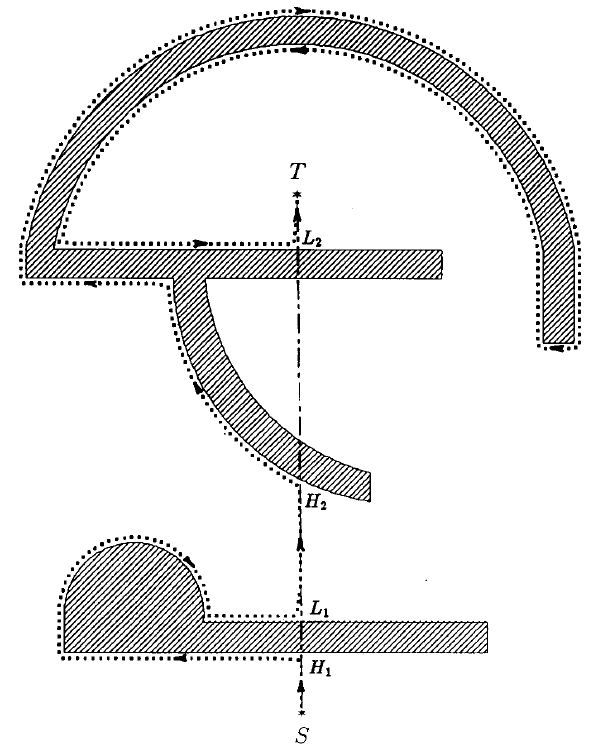
\includegraphics[height = 9cm]{Images/Bug2}     
			\caption{Demonstration of the Bug2 algorithm (Image taken from \cite{Lumelsky1990})}
			\label{IM_Bug2}
		\end{figure}
		
		\subsubsection{Potential Field Method}\label{SSECT_PotentialField}
		Another widely used and documented algorithm is the potential field method. This method works on the basis of creating attractive potentials, in the form of goals and unattractive potentials, which can be the obstacles or no fly zones. A simple way of describing this method is to make a comparison with a charged particle moving through a potential field. In this case, the aircraft is considered a positive charge and the end goal or position is considered a negative charge. The goal will provide an attraction force based on the robot's proximity to the end point. Obstacles, in this analogy, can then be thought of as other positive particles which will produce a negative, or repelling force to the platform. The algorithm will then calculate the attractive and repelling forces based on immediate sensing data. The sum of all of these forces can then be given to the craft and used as a command to allow for successful navigation in an unknown environment.
		
		An important consideration is the generation of these forces based on simple proximity measurements. Traditionally there will be a single goal which will attract with a parabolic like force, that increases quadratically as the robot moves further away from the goal. This set up will also ensure that the force felt by the robot decreases as the setpoint is approaching, limiting overshoot in the final system. Although the platform can expect one goal, there might be multiple objects in it's vicinity all creating repelling forces. The repelling force is then calculated by summing all of these forces.
		
		A major limitation of the potential field method is the assumed holonomy of the platform. A non-holonomic vehicle will struggle to implement a potential field method as the direction of the induced forces may not be reachable for the platform in given scenarios. Another downfall of this method is the local minima created when the sum of repulsion forces equals to the sum of attractive forces. Figure \ref{IM_LocalMinima} is used to illustrate a scenario where this local minima is created. Careful sensor placement can limit the occurrence of these situations, however it will be virtually impossible to remove this risk completely.
		
		\begin{figure}[H]
			\centering
			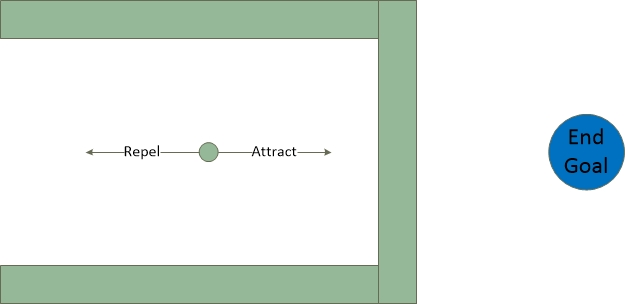
\includegraphics[height = 6cm]{../References/Diagrams/LocalMinima}     
			\caption{Local minima seen with potential field method}
			\label{IM_LocalMinima}
		\end{figure}
		
	
	
	
